\section{High Energy Physics Applications}

We study applications taken from two experiments of the CERN Large Hadron Collider, namely the ATLAS experiment and the CMS experiment. 
One of the applications of the ATLAS experiment is the \emph{Athena} application, which is a general purpose processing framework including algorithms
for event reconstruction and data reduction \cite{calafiura2005athena}. The CMS experiment is conducted through an application termed  \emph{TauRoast}, which searches for specific 
cases where the Higgs boson decays to two tau leptons~\cite{chatrchyan2013search}. In LHC, the ATLAS and CMS experiments are distinct, 
developed independently by two entirely separate physics communities. Consequently, their applications  
have very different software distribution and data management frameworks, making it interesting to examine if common reproducibility frameworks and 
tools work across the two communities. 

Code and data in \emph{TauRoast} is available through five different networked filesystems, namely an HDFS cluster for data files, 
some configuration files were stored on a CVMFS~\cite{blomer2011cernvm} filesystem, and a variety of software tools were on an NFS, PanFS and AFS systems.
In addition, code may exist in version control systems such as Git, CVS, and CMS Software Distribution (CMSSW). %~\cite{cms2006cms}. 
\begin{wrapfigure}{r}{0.4\textwidth}
\small
\centering
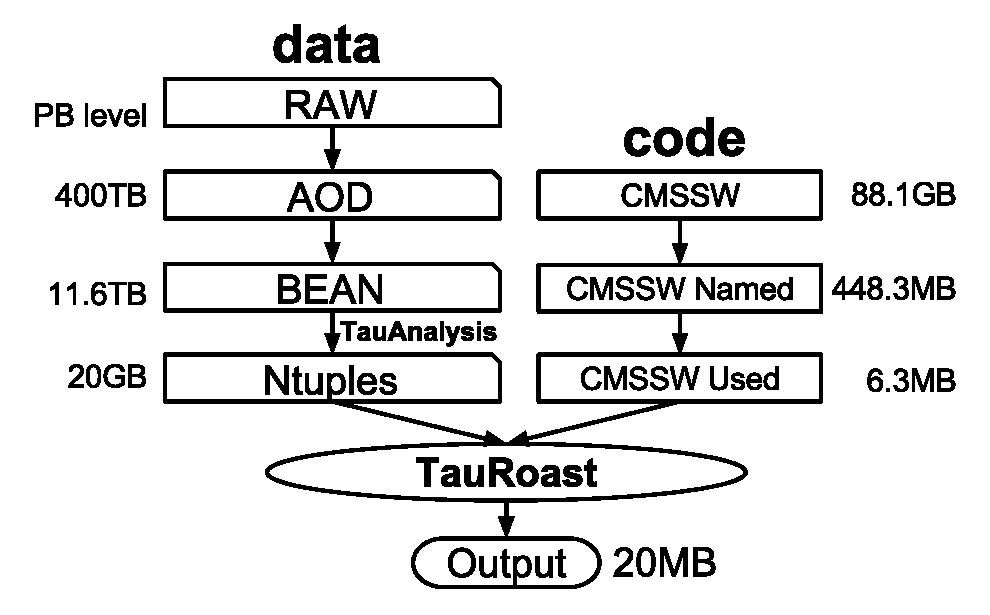
\includegraphics[width=.4\textwidth]{data-code-size.eps}
\caption{Inputs to Tau Roast}
\label{fig:data-code-size}
\end{wrapfigure}
Data that is input to \emph{TauRoast} is obtained by reducing it through a pipeline, as shown in Figure \ref{fig:data-code-size}. Consequently, the real input data may 
vary depending upon the science question being researched. Similarly the software may name many possible components but the used components are
smaller than the named ones. 

In \emph{Athena} data is obtained through an external Dropbox-like system called the FaxBox, but does not go through any reduction steps. Code is obtained through 
CVMFS, which provides the analysis routines. However, depending upon the input data code and the configuration that will be invoked changes. 
Thus in \emph{Athena} the used code and configuration are dynamic depending upon input data, where as in \emph{TauRoast} the code and data are static, 
but the amount of data and code to include changes depending on the involved science. 

